% !TEX TS-program = lualatex
% !TEX encoding = UTF-8 Unicode

\documentclass[12pt, letterpaper]{article}

%%BIBLIOGRAPHY- This uses biber/biblatex to generate bibliographies according to the
%%Unified Style Sheet for Linguistics
\usepackage[main=american, german]{babel}% Recommended
\usepackage{csquotes}% Recommended
\usepackage[backend=biber,
        style=unified,
        maxcitenames=3,
        maxbibnames=99,
        natbib,
        url=false]{biblatex}
\addbibresource{.bib}
\setcounter{biburlnumpenalty}{100}  % allow URL breaks at numbers
% \setcounter{biburlucpenalty}{100}   % allow URL breaks at uppercase letters
% \setcounter{biburllcpenalty}{100}   % allow URL breaks at lowercase letters

%%TYPOLOGY
\usepackage[svgnames]{xcolor} % Specify colors by their 'svgnames', for a full list of all colors available see here: http://www.latextemplates.com/svgnames-colors
\usepackage[hmargin=1in,vmargin=1in]{geometry}  %Margins          
\usepackage{graphicx}	%Inserting graphics, pictures, images 		
\usepackage{stackengine} %Package to allow text above or below other text, Also helpful for HG weights 
\usepackage{fontspec} %Selection of fonts must be ran in XeLaTeX or LuaLateX
\usepackage{amssymb} %Math symbols
\usepackage{amsmath} % Mathematical enhancements for LaTeX
\usepackage{setspace} %Linespacing
\usepackage{multicol} %Multicolumn text
\usepackage{enumitem} %Allows for continuous numbering of lists over examples, etc.
\usepackage{multirow} %Useful for combining cells in tablesbrew 
\usepackage{hanging}
\usepackage{fancyhdr} %Allows for the 

\pagestyle{fancy}
\fancyhead[L]{\textit{LING 450/550}} 
\fancyhead[R]{Autumn 2025} 
\fancyfoot[L]{Updated: \textit{\today}} 
\fancyfoot[C]{}
\fancyfoot[R]{\thepage} 
\renewcommand{\headrulewidth}{0.4pt}
\setlength{\headheight}{14.5pt} % ...at least 14.49998pt
% \usepackage{fourier} % This allows for the use of certain wingdings like bombs, frowns, etc.
% \usepackage{fourier-orns} %More useful symbols like bombs and jolly-roger, mostly for OT
\usepackage[colorlinks,allcolors={black},urlcolor={blue}]{hyperref} %allows for hyperlinks and pdf bookmarks
% \usepackage{url} %allows for urls
% \def\UrlBreaks{\do\/\do-} %allows for urls to be broken up
\usepackage[normalem]{ulem} %strike out text. Handy for syntax
\usepackage{tcolorbox}
\usepackage{datetime2}
\usepackage{longtable}
\usepackage{booktabs}

%%FONTS
\setmainfont{Libertinus Serif}
\setsansfont{Libertinus Sans}
\setmonofont[Scale=MatchLowercase]{Libertinus Mono}

%%PACKAGES FOR LINGUISTICS
\usepackage[noipa]{OTtablx} % Use this one generating tableaux without using TIPA
\usepackage{langsci-gb4e} % Language Science Press' modification of gb4e
\usepackage{tikz} % Drawing Hasse diagrams
\usepackage{leipzig} %	Offers support for Leipzig Glossing Rules

%%LEIPZIG GLOSSING FOR ZAPOTEC
\newleipzig{el}{el}{elder} % Elder pronouns
\newleipzig{hu}{hu}{human} % Human pronouns
\newleipzig{an}{an}{animate} % Animate pronouns
\newleipzig{in}{in}{inanimate} % Inanimate pronouns
\newleipzig{pot}{pot}{potential} % Potential Aspect
\newleipzig{cont}{cont}{continuative} % Continuative Aspect
\newleipzig{stat}{stat}{stative} % Stative Aspect
\newleipzig{and}{and}{andative} % Andative Aspect
\newleipzig{ven}{ven}{venative} % Venative Aspect
% \newleipzig{res}{res}{restitutive} % Restitutive Aspect
\newleipzig{rep}{rep}{repetitive} % Repetitive Aspect

%%TITLE INFORMATION
\title{TITLE}
\author{Mykel Loren Brinkerhoff}
\date{\today}

%%MACROS
\newcommand{\sub}[1]{\textsubscript{#1}}
\newcommand{\supr}[1]{\textsuperscript{#1}}

\makeatletter
\renewcommand{\paragraph}{%
  \@startsection{paragraph}{4}%
  {\z@}{0ex \@plus 1ex \@minus .2ex}{-1em}%
  {\normalfont\normalsize\bfseries}%
}
\makeatother
\parindent=10pt


\begin{document}

%%If using linguex, need the following commands to get correct LSA style spacing
%% these have to be after  \begin{document}
    % \setlength{\Extopsep}{6pt}
    % \setlength{\Exlabelsep}{9pt}		%effect of 0.4in indent from left text edge
%%

%% Line spacing setting. Comment out the line spacing you do not need. Comment out all if you want single spacing.
%	\doublespacing
%	\onehalfspacing

\begin{center}
     {\Large \textbf{Ultrasound and IPA}}
\end{center}
%\maketitle
%\maketitleinst
% \thispagestyle{fancy}

% \tableofcontents

%------------------------------------
\section*{Consonants} \label{}
%------------------------------------

\vspace*{\fill}
\begin{center}
    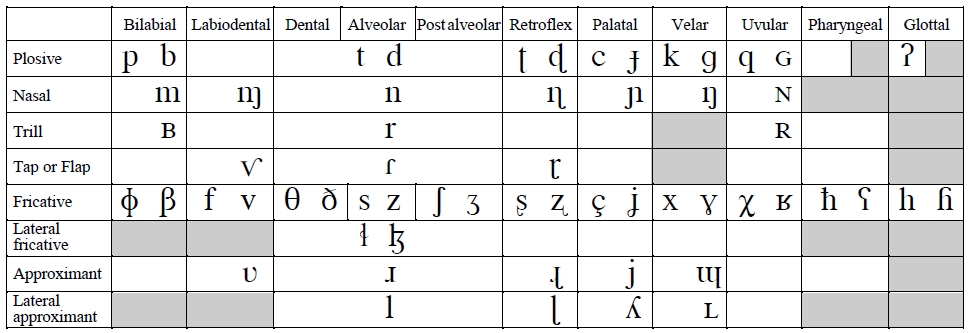
\includegraphics[width = \textwidth]{figs/IPAConsonants.png}
\end{center}
\vspace*{\fill}

\newpage
%------------------------------------
\section*{Vowels} \label{}
%------------------------------------

\vspace*{\fill}
\begin{center}
    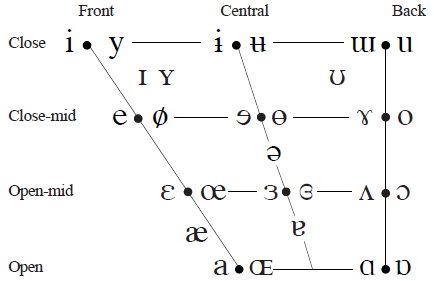
\includegraphics[width = 0.75\textwidth]{figs/IPAVowels.png}
\end{center}
\vspace*{\fill}

%------------------------------------
%\section{} \label{}
%------------------------------------


%------------------------------------
%\section{} \label{}
%------------------------------------


%------------------------------------
%BIBLIOGRAPHY
%------------------------------------

%\singlespacing
%\nocite{*}
\printbibliography[heading=bibintoc]

\end{document}